\chapter{Experiment}\label{ch:exp}
	This chapter describes in detail the implementation and experimental setup of the overall framework used in this thesis. In addition, Section \ref{sec:dataset} discusses in depth about the dataset of steel type plate images, the process of creating image pairs and synthetic data elaborately. Finally, Section \ref{sec:eval} describes the evaluation metrics used to measure the performances of all the GANs and OCR engines under study.

\section{Implementation}\label{sec:imp}
In this section, we list out the best hyperparameters for each method from the different settings that were tried out and their implementation in detail. For all the three GANs that were studied, we used the ADAM optimizer with the same values $\beta_1$ 0.5 and $\beta_2$ 0.999 for both generator and discriminator. We have used the PatchGAN discriminator for both pix2pix and CycleGAN experiments. We have performed experiments with different combinations for hyperparameters such as\\
i) Normalization \\
ii) Regularization using dropout \\
iii) Batch size with respect to multiple GPUs \\
iv) Size of the input image\\
v) Data augmentation using flip\\
vi) Learning rate\\
vii) Use of synthetic data\\
viii) Architecture for generator and discriminator\\

	The random search with qualitative evaluation was used for hyperparameter optimization. Many hyperparameters such as batch size, epoch, etc had little impact on the results of the training. For all the three GANs, the combination of parameters used in the original paper produced the best results. These settings are listed in the following table:

\begin{table}[H]
\resizebox{\textwidth}{!}{%
\begin{tabular}{@{}|c|c|c|c|@{}}
\toprule
                       & \textbf{Pix2pix}    & \textbf{CycleGAN}   & \textbf{FactorGAN}          \\ \midrule
\textbf{Batch Size}    & 4      & 2        & 25       \\ \midrule
\textbf{Learning Rate} & 0.002  & 0.002    & 0.001    \\ \midrule
\textbf{Optimizer}     & Adam   & Adam     & Adam     \\ \midrule
\textbf{beta1}         & 0.5    & 0.5      & 0.5      \\ \midrule
\textbf{beta2}         & 0.999  & 0.999    & 0.999    \\ \midrule
\textbf{Epoch}         & 200    & 200      & 200      \\ \midrule
\textbf{Dropout}       & No     & Yes      & No       \\ \midrule
\textbf{Normalization} & Batch  & Instance & Spectral \\ \midrule
\textbf{Generator}     & ResNet & ResNet   & U-Net     \\ \midrule
\textbf{Discriminator} & Patch discriminator & Patch discriminator & Convolutional discriminator \\ \bottomrule
\end{tabular}%
}
\caption{Best parameter setting used in the experiments for each GAN}
\label{tab:tabparam}
\end{table}

The original PyTorch implementation of GAN and OCR models that have been used for training can be found in the following repositories :
\newline
\begin{enumerate}
\item \textbf{Pix2pix \& CycleGAN} - \url{https://github.com/junyanz/pytorch-CycleGAN-and-pix2pix}

\item \textbf{FactorGAN} - \url{https://github.com/f90/FactorGAN}

\item \textbf{Text detection} - \url{https://github.com/clovaai/CRAFT-pytorch}

\item \textbf{Text detection pretrained model (craft-mlt-25k.pth)} - \url{https://drive.google.com/file/d/1Jk4eGD7crsqCCg9C9VjCLkMN3ze8kutZ/view}

\item \textbf{Text recognition} - \url{https://github.com/clovaai/deep-text-recognition-benchmark}

\item \textbf{TPS-ResNet-BiLSTM-Attn.pth} - The pretrained model for text recognition can be found in \url{https://drive.google.com/drive/folders/15WPsuPJDCzhp2SvYZLRj8mAlT3zmoAMW}
\end{enumerate}

	All the codes used in the thesis, latex files and the codes that are referenced from public repositories along with its respective licenses are included in the university GitLab repository. It can be cloned using the following URL: \url{https://www.uni-hildesheim.de/gitlab/panneers/thesis_steel_type_plate_recognition.git}.

\section{Experimental setup}
For our experiments, all codes are written in python and implemented in PyTorch. We have used other python libraries such as Numpy, Scipy, Pillow, Scikit-Learn. For training, we have used machines with a configuration having AMD Ryzen TR 2920X processor with 64 cores, 2 x 8 GB RTX 2070 Super X GPU, 128 GB RAM.

\section{Dataset}\label{sec:dataset}

This section provides a brief description of the dataset used in this thesis. Generally, the datasets for everyday objects are widely available. But for specific industrial use cases like in our case, it remains scarce. So, the data needs to be created from scratch.

\subsection{Data collection}
	Here, we introduce our strategies to dataset collection and processing. The following steps were performed to create the dataset:
\begin{enumerate}
\item A python script is written such that it crawls the steel type plate images from the google image search to create the dataset. 
\item Then the resulting images of web scraping were manually refined to remove the unnecessary images from the dataset. 
\item The images were cropped to remove the background information and to keep only the steel type plates part in the image.
\item In the middle of the experiment, few duplicate images were found in the dataset. Then these duplicate images were removed using a python script.
\item All the images in the dataset were resized to a uniform resolution of 600 x 400.
\item The final dataset consists of train, test and validation split with 366 in the train set, 30 in the validation set and 100 images for the testing set.
\end{enumerate}

\subsection{Label creation}
Since we use the image-to-image translation GAN models, the target labels corresponding to each input image needed to be created for training. The labels for every image is created in the following manner :

\begin{itemize}

\item Initially the RGB images in the dataset are converted to grayscale images.

\begin{figure}[H]
\centering
\begin{subfigure}{.47\textwidth}
  \centering
  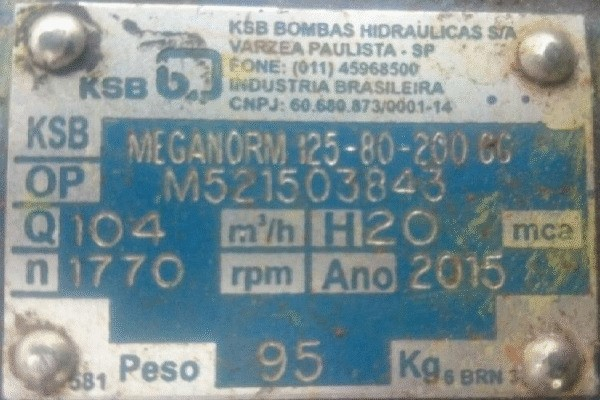
\includegraphics[width=.7\linewidth]{images/L1.jpg}
  \caption{RGB image}
\end{subfigure}%
{\LARGE$\xrightarrow{}$}%
\begin{subfigure}{.47\textwidth}
  \centering
  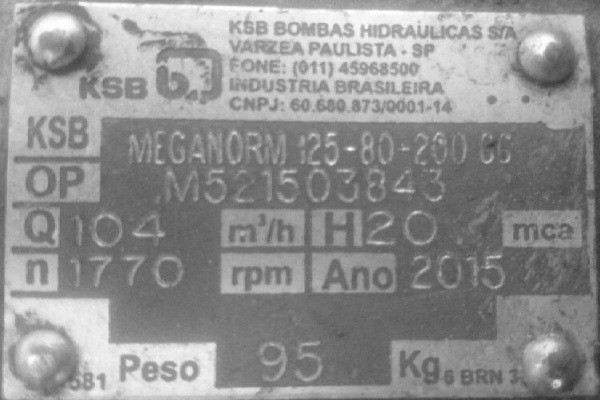
\includegraphics[width=.7\linewidth]{images/L2.jpg}
  \caption{Grayscale image}
\end{subfigure}
\caption{RGB to Grayscale conversion}
\end{figure}

\item Then, we used the \textit{Photo Sketch} app in the iPad and highlighted the text part on top of each grayscale image manually using Apple pencil as shown in Figure \ref{fig:ann}. 

\begin{figure}[H]
\centering
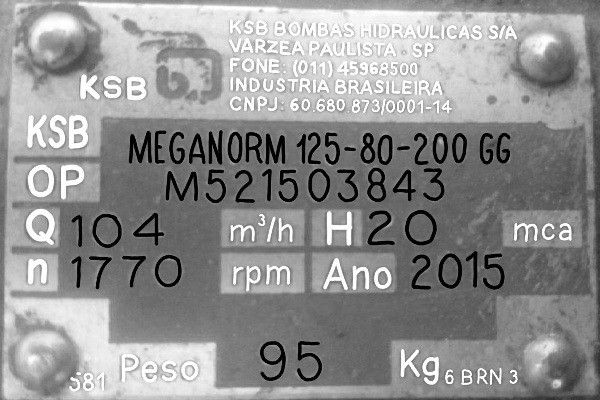
\includegraphics[width=3in]{images/L3.jpg}
\caption{Annotated image}
\label{fig:ann}
\end{figure}

\item Now, the difference is calculated between the annotated image and the grayscale image using \textit{ImageOps} function from the Pillow library. The resulting image is shown in Figure \ref{fig:diff}.

\begin{figure}[H]
\centering
\begin{subfigure}{.49\textwidth}
  \centering
  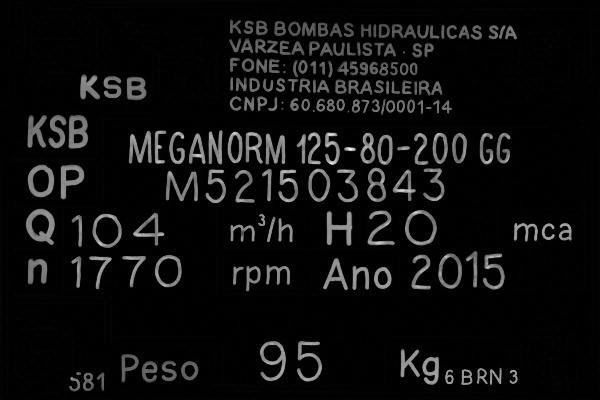
\includegraphics[width=.9\linewidth]{images/L4.jpg}
  \caption{Difference image}
  \label{fig:diff}
\end{subfigure}%
\begin{subfigure}{.49\textwidth}
  \centering
  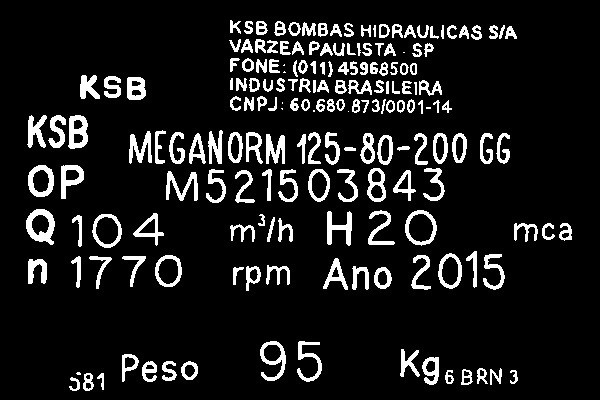
\includegraphics[width=.9\linewidth]{images/L5.jpg}
  \caption{Binary image}
  \label{fig:thres}
\end{subfigure}
\caption{The resulting image with better constrast between text and background}
\end{figure}

\item Finally the binary image is produced using an \textit{Adaptive Thresholding} function from the python OpenCV library. But thresholding step is skipped during training since it seemed to produce more noise in the translation results.

\begin{figure}[H]
\centering
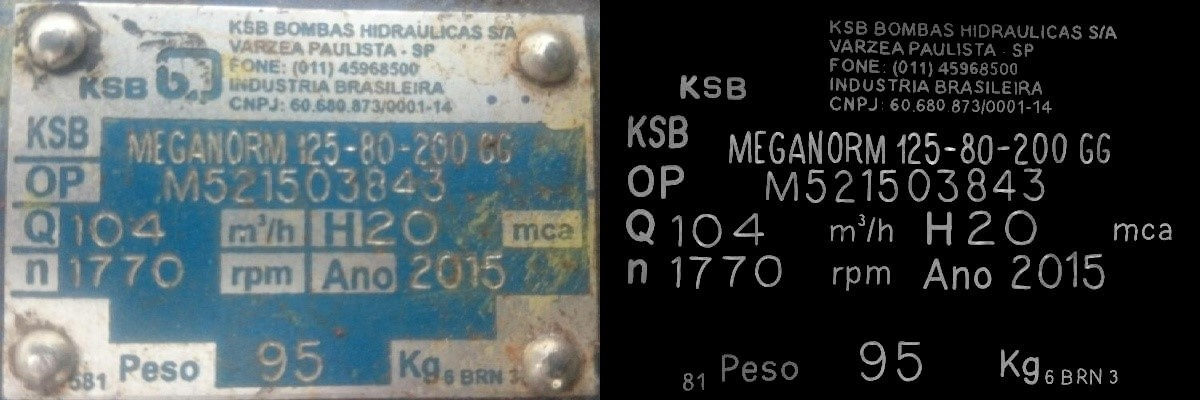
\includegraphics[width=5in]{images/imagepair.jpg}
\caption{A steel type plate image with its input and output pair}
\label{fig:imgpair}
\end{figure}
\end{itemize}

	The final image pair sample used for training is shown in Figure \ref{fig:imgpair}.
\subsection{Synthetic dataset}
A framework to create a synthetic dataset is introduced in this thesis to generate images close to real steel type plates. The synthetic data supplement the original dataset since it has less than 400 image pairs and helps in reducing the manual effort of annotating more images.
\newline
\begin{wrapfigure}{r}{0.5\textwidth}
\centering
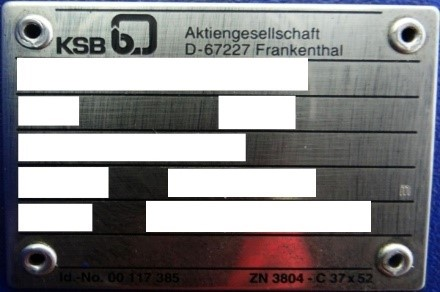
\includegraphics[width=0.4\textwidth]{images/template.jpg}
\caption{A sample template image}
\label{fig:template}
\end{wrapfigure}

	The Figure \ref{fig:template} shows a steel type plate template. More such templates are available for selection in the framework. The dictionary pool consists of around 750 image patches that contain different shapes of alphanumeric characters as well as word patches randomly cropped from the original images of steel type plates with its corresponding labels. Figure \ref{fig:syndata} shows some of the samples of cropped image patches present in the dictionary with its output pair.
\begin{figure}[H]
\centering
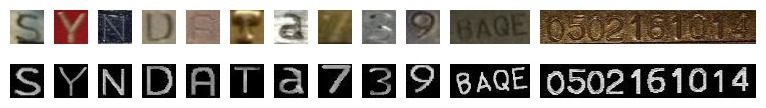
\includegraphics[width=5in]{images/syndata.jpg}
\caption{Sample image pairs in the dictionary pool}
\label{fig:syndata}
\end{figure}

The framework is built using python script and OpenCV libraries. At first, it randomly chooses a template of the steel plate. Once the template is selected, the framework loads the objects of the selected template class. 
\newline
\begin{figure}[H]
\centering
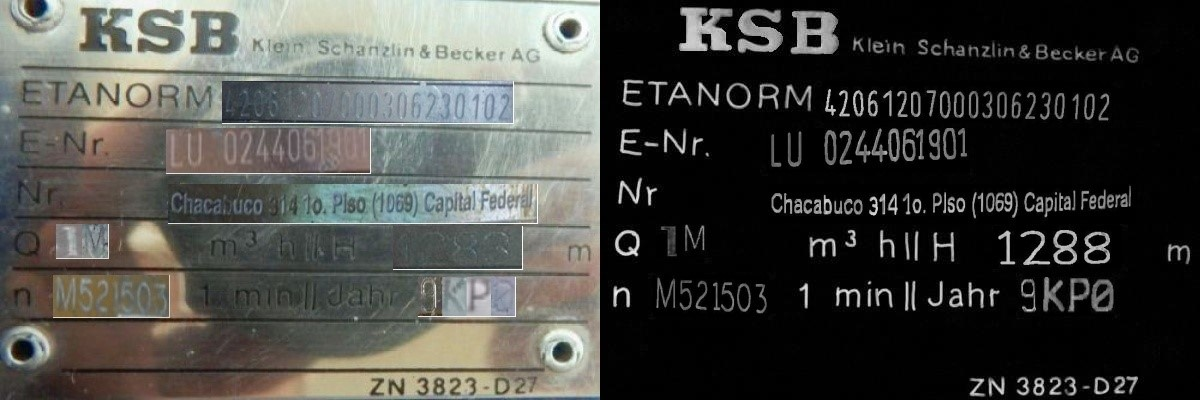
\includegraphics[width=5in]{images/synda1.jpg}
\caption{A synthetic image with its input and output pair}
\label{fig:syn}
\end{figure}

	It contains information such as the location of the templates, number of cropped areas and corresponding bounding box coordinates. Then, the framework picks a random item from the dictionary and fits these into each white boxes of the template. The generated synthetic image is shown in Figure \ref{fig:syn}. The framework has the option to vary the illumination and brightness of the generated image. Furthermore, it also has the functionality to add noises like gaussian, speckle, salt \& pepper, etc. 

\section{Evaluation metrics}\label{sec:eval}
The evaluation of the generative models is still an open research problem \citep{salimans2016improved}. The GAN generates realistically synthetic images and is often difficult to compare the performance of different GAN models with one another. \cite{borji2019pros} in their work, conducted a detailed study on the evaluation of GAN. According to their research, several methods have been introduced to evaluate GAN  yet there is no clear winner on which method captures the strengths and limitations of the model.
	The evaluation methods for GAN can be generally classified into two types: i) Quantitative evaluation and ii) Qualitative  evaluation

\subsection{Quantitative evaluation}
\cite{yang2018mri} used metrics such as \gls{mae}, \gls{psnr} to evaluate their work of image-to-image translation model. Similarly in this thesis, we have used MSE, SSIM and FID score to quantitatively measure the performance of the different GAN models. The synthetic images can be quantitatively evaluated with metrics such as MSE that calculate per-pixel-errors. This method calculates the average pixel difference between the ground truth images and the generated images. The MSE is not a great measure for performance indicators since it does not reveal anything about the quality or structural similarity of the image. Yet, higher MSE means the generated image is very different from the ground truth image. The MSE of two images x and y is given by

\begin{equation*}
MSE(x,y) = \frac{1}{m*n}\sum_{i=0}^{m-1}\sum_{j=0}^{n-1}[x(m,n) - y(m,n)]^2
\end{equation*}

SSIM proposed by \cite{wang2004image} can be used to measure the similarity and quality of generated images with respect to the ground truth. It compares the pixels of two images using three quantities such as luminance (I), contrast (C) and structure (S). For images x and y , it is given by,

\begin{align*}
I(x,y) = \dfrac{2\mu_x\mu_y + C_1}{\mu^2_x + \mu^2_y + C_1} \;\;\;
C(x,y) = \dfrac{2\sigma_x\sigma_y + C_2}{\sigma^2_x + \sigma^2_y + C_2} \;\;\;
S(x,y) = \dfrac{\sigma_{xy} + C_3}{\sigma_x \sigma_y + C_3}
\end{align*}

	where, $\mu_x,\mu_y,\sigma_x \; and \; \sigma_y$ denote the mean and standard deviation of pixel intensities between two images. $C_1, C_2 \; and \; C_3$ are constants added for numerical stability. The final SSIM score \citep{wang2004image} is given by
	
\begin{equation*}
SSIM(x,y) = I(x,y)^\alpha C(x,y)^\beta S(x,y)^\gamma
\end{equation*}

	where $\alpha, \beta \; and \; \gamma$ are the parameters to adjust the relative importance of I, C and S. The score ranges between 0 (Low similarity) and 1 (High similarity).

\subsection*{Frechet Inception Distance (FID)}
	The most commonly used method to evaluate the quality of generated images is to use classifiers pre-trained on real image distribution. Inception score is a measure that classifies if the synthetic images are realistic with the help of a classification network trained on real images. \citeauthor{heusel2017gans} proposed FID which is an improvised version of the Inception score. FID compares the Gaussian distribution of ground truth with generated images to quantify its quality. The FID score between real and generated images \citep{heusel2017gans} is given by 

\begin{equation*}
FID(r,g) = \lVert{\mu_r - \mu_g}\lVert_2^2 \; +  \; T_r(\Sigma_r + \Sigma_g - 2(\Sigma_r\Sigma_g)^{\frac{1}{2}})
\end{equation*}
	
It is shown that the FID score is more reliable, consistent and robust than the Inception score. Lower the FID score, better the quality of generated images.

\subsection{Qualitative evaluation}
The manual image inspection is a good starting point for qualitative analysis although visual comparison of real and generated images is difficult when the changes are very small.
The qualitative evaluation is not sufficient to determine the performance of the GAN. Therefore it is used together with the other metrics to evaluate the synthetic images such that it complements the quantitative evaluation. In this thesis, the synthetic image generated by three different GANs under study is visually distinguishable.
\subsection{Evaluation of OCR}
	For evaluating the OCR engines, we have conducted experiments with the test images before translation as well as the corresponding GAN translated images. These images are passed separately to both the proposed OCR engine and the commercial OCR tool like Google Vision. Finally, we have two outcomes for each OCR engine: i) character recognition of images without GAN translation and ii) character recognition of images using GAN translation. Then the output is compared with the annotations and the results are tabulated. We take into measures like the number of characters present in the text, the number of characters identified and the recognition rate in the name of OCR score. The OCR score is given by the number of characters identified correctly divided by the total number of texts present in the image. 
The following formula is used to calculate the OCR score: 
\begin{align*}
OCR \; score = \dfrac{Total \; number \; of \; characters \; identified \; correctly}{Total \; number \; of \; characters} * 100
\end{align*}
